%
%  monografia
%
%  Created by Ricardo de Cillo on 2012-05-27.
%  Copyright (c) 2012 __MyCompanyName__. All rights reserved.
%
\documentclass[a4paper,11pt]{article}

% Use utf-8 encoding for foreign characters
\usepackage[brazil]{babel}
\usepackage[utf8]{inputenc}
\usepackage[T1]{fontenc}

% Setup for fullpage use
\usepackage{fullpage}
\usepackage{setspace}

% Uncomment some of the following if you use the features
%
% Running Headers and footers
%\usepackage{fancyhdr}

% Multipart figures
%\usepackage{subfigure}

% More symbols
\usepackage{amsfonts}
\usepackage{amssymb, amsmath}
%\usepackage{latexsym}

% Surround parts of graphics with box
\usepackage{boxedminipage}

% Package for including code in the document
\usepackage{listings}

% If you want to generate a toc for each chapter (use with book)
\usepackage{minitoc}

% This is now the recommended way for checking for PDFLaTeX:
\usepackage{ifpdf}

%\newif\ifpdf
%\ifx\pdfoutput\undefined
%\pdffalse % we are not running PDFLaTeX
%\else
%\pdfoutput=1 % we are running PDFLaTeX
%\pdftrue
%\fi

\ifpdf
\usepackage[pdftex]{graphicx}
\else
\usepackage{graphicx}
\fi


\usepackage{xcolor}
\newcommand{\TODO}[1]{\textcolor{red}{#1}}


%% \title{Aplicação de análise morfológica para segmentação de páginas em imagens de documentos}
%% \author{ Aluno: Ricardo de Cillo \\ Supervisora: Nina S. T. Hirata }

% \date{2012-05-27}

\begin{document}

%  \maketitle

% =======================================================================
% CAPA
% =======================================================================

\thispagestyle{empty}
\

\

\

\

\begin{center}
{\bf \Large Trabalho de Formatura Supervisionado}

\bigskip
\bigskip
{\bf \LARGE Aplicação de análise morfológica para segmentação de páginas em imagens de documentos}

\bigskip
{\large Ricardo de Cillo}

\bigskip
Supervisora: Nina S. T. Hirata 

\bigskip
Departamento de Ciência da Computação\\
Intituto de Matemática e Estatística, IME-USP
\end{center}


\bigskip
\begin{quote}
\begin{spacing}{1.2}
\noindent {\bf \large Resumo}: Neste texto apresentaremos nosso estudo sobre métodos morfológicos aplicados à segmentação de páginas, etapa importante na análise de documentos que busca extrair informações sobre a sua estrutura: regiões com títulos, legendas, figuras e blocos de texto. A qualidade da solução obtida será medida e comparada, segundo os mesmo critérios aplicados à resultados considerados estado da arte por pesquisadores da área.
\end{spacing} 
\end{quote}

% Uma das aplicações da teoria de visão computacional é a análise de imagens de documentos. O objetivo desta aplicação é extrair informações sobre o conteúdo e estrutura de um documento digitalizado. Uma das etapas envolvidas é a segmentação de página que consiste na identificação de áreas da imagem correspondentes à elementos estruturais, tais como títulos, legendas e blocos de texto. Nesta monografia iremos explorar métodos morfológicos aplicados à segmentação de páginas. A qualidade da solução obtida será medida e comparada, segundo os mesmo critérios aplicados à resultados considerados estado da arte por pesquisadores da área.


% Este trabalho é sobre segmentação automática de documentos, ou seja, dado um documento digitalizado - revista, jornal, artigo científico, documento histórico entre outros - extrairemos informações sobre sua estrutura (blocos de texto, figuras, gráficos, títulos. Dentre as tecnicas utilizadas teremos operadores morfológicos e aprendizado computacional. Também fizemos um comparativo com as soluções consideradas estado da arte por pesquisadores da área. 

\bigskip
\begin{center}
São Paulo, \today
\end{center}



\newpage
\setcounter{page}{1}



\section{Introdução}

\cite{Nina:2010a} \cite{trios:online} \cite{DBLP:conf/icdar/2009}

Processamento e análise de documentos é uma importante subárea da área
de reconhecimento de padrões cujo principal objetivo é a
interpretação de um documento, ou seja, o entendimento
da sua estrutura bem como o reconhecimento de cada um dos
componentes estruturais.

\begin{figure*}[htb]
\begin{center}
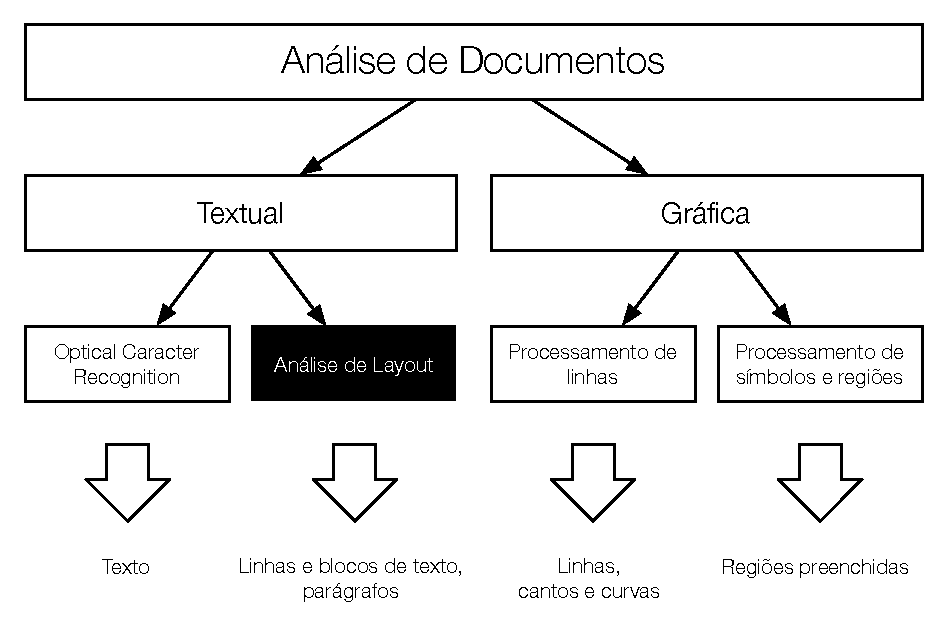
\includegraphics[width=0.7\textwidth]{assets/document_processing_areas_hierarquies.pdf}
\end{center}
\caption{Contextualização do tema do trabalho entre as áreas da
  análise de documentos. Adaptado de~\cite{Kasturi_OGorman_Govindaraju_2002}}
\label{fig:context1}
\end{figure*}

Segmentação de página refere-se à tarefa de separar e rotular os diferentes
componentes que fazem parte da estrutura das páginas de
documento, tais como: blocos de texto, gráficos, figuras, títulos,
legendas, separadores, tabelas, fórmulas matemáticas e regiões com
ruído.

Em geral, a segmentação de página é um dos primeiros passos no
processo de entendimento de um documento. Uma vez identificiados os
blocos estruturais, processamentos específicos para cada tipo de bloco
podem ser aplicados. Por exemplo, no caso de blocos de textos é
conveniente fazer o reconhecimento de texto para que o mesmo possa ser
armazenado em formato texto (e não imagem). Por outro lado, no caso de
imagens, pode ser interessante armazená-las em alta resolução para
manter a qualidade. Documentos digitalizados podem ser processados
eficientemente em processos que envolvem armazenamento, edição,
transmissão, ou busca, por exemplo.

Devido à grande quantidade de documentos, é interessante que o seu
processamento seja realizado de forma automatizada ou pelo menos
semi-automatizada. Para tal, diversas soluções computacionais vêm
sendo propostas para o problema ao longo dos anos desde o surgimento
desse campo de pesquisa. Automatizar esta tarefa reduz custos, aumenta
a velocidade e capacidade de processamento de documentos além de
possivelmente reduzir a taxa de erro humano na classificação de uma
região.

Neste trabalho exploraremos a aplicabilidade de operadores
morfológicos automaticamente gerados ao problema de segmentação de
páginas.

Este texto está organizado da seguinte forma. Na seção~\ref{sec:fundamentos},
apresentamos as definições e conceitos básicos que serão importantes
para a leitura deste texto.

\section{Fundamentos}
\label{sec:fundamentos}

\subsection{Imagens digitais}
  Uma imagem digital monocromática pode ser definida como uma função $f:
  \mathbb{E} \subset \mathbb{Z}^2 \to \mathbb{K} = \{0,1,\ldots,k-1\}$, na qual $k$ representa o número de tons de cinza. Tipicamente adota-se $k=256$, ou seja, 8-bits de cor. Quando $k=1$ as imagens são denominadas {\bf binárias}; quando $k>1$ as imagens são denominadas {\bf tons de cinza}. Na prática, o domínio $\mathbb{E}$ é um retângulo finito de dimensões $m\times n$ (uma matriz de $m$ linhas e $n$ colunas).

  Uma imagem RGB (colorida) é uma função $f: \mathbb{E} \to \mathbb{K}^3$.

\subsection{Operadores de imagens}
Um operador de imagens é uma função que mapeia imagens em
imagens. Denotando $\mathbb{E}=\mathbb{Z}^2$, $K=\{0,1,\ldots,k-1\}$ e
todas as imagens definidas em $\mathbb{E}$ por $K^{\mathbb{E}}$,
  podemos representar um operador de imagens como $\Psi: K^{\mathbb{E}}
    \to K^{\mathbb{E}}$.

\subsubsection{Binarização de imagens}

A classe de operadores morfológicos estudada restringe-se ao domínio das imagens binárias. Porém as imagens obtidas através de digitalização usualmente são coloridas (RGB de 24-bits). O processo de binarização é realizado por um operador que mapeia uma imagem colorida ou monocromática em uma imagem binária.

Neste trabalho, primeiramente transformamos as imagens coloridas para níveis de cinza e posteriormente aplicamos a binarização.

Existem muitos algoritmos que realizam esta tarefa. Uma revisão extensa dos mais conhecidos métodos de binarização é apresentada em \cite{citeulike:890354}. Todos eles se aplicam a imagens em níveis de cinza, portanto inicialmente transformaremos a imagem colorida $f$ em níveis de cinza $g$:

\begin{equation}
  f(x) = \mathbb{K}^3 \rightsquigarrow g(x) = \mathbb{K} \rightsquigarrow b(x) = \{0, 1\}
\end{equation}

\subsection{Classificação de objetos}

Na área de reconhecimento de padrões e aprendizado computacional
estudam-se métodos e técnicas para classificação de dados em geral. Os
dados (padrões) a serem classificados correspondem, em geral, à
representação digital de algum objeto concreto ou abstrato. O objetivo
da classificação é atribuir um rótulo de classe a cada padrão
observado.

Dependendo do problema, os rótulos de classe podem ser conhecidos ou
não. Por exemplo, se desejamos fazer o reconhecimento de caracteres,
os padrões são a imagem dos caracteres e os rótulos de classe são as
identificações dos possíveis caracteres. Por outro lado, em problemas
como na classificação de perfil de consumidores, pode não haver um
conjunto de perfis pré-estabelecidos e o objetivo seria então
identificar a possível existência de perfis. O primeiro é conhecido
como problema de classificação supervisionada e o segundo como
classificação não-supervisionada.

No caso da classificação supervisionada, supõe-se que os padrões são
elementos de um espaço $X$ e que o conjunto de rótulo de classe é dado
por $Y=\{y_1,y_2,\ldots,y_c\}$. Assim, um classificador pode ser
expresso por uma função $f: X \to Y$.

Frequentemente $X$ é um subespaço de $\mathbb{R}^d$. Assim, um padrão
é representado por uma $d$-upla $\mathbf{x}=(x_1,x_2,\ldots,x_d) \in
\mathbb{R}^d$.

\subsection{Segmentação de imagens}

A segmentação de imagens é um processamento comum a praticamente
todos os processos que envolvem análise de imagens. Segmentar uma
imagem corresponde a particionar o seu domínio, de forma que cada
região resultante corresponda (do ponto de vista semântico) a uma
componente de interesse na análise em questão. Este problema pode ser modelado como uma classificação de objetos, onde o conjunto de pixels de uma imagem são os objetos em $X$ e as componentes em $Y$ são regiões de interesse, como ilustrado na tabela \ref{tab:image_segmentation}.

\begin{table}
  \caption{Exemplo de segmentação de imagem: separando frente e fundo.}
  \begin{tabular}[p]{@{}ccc@{}}
    \centering
    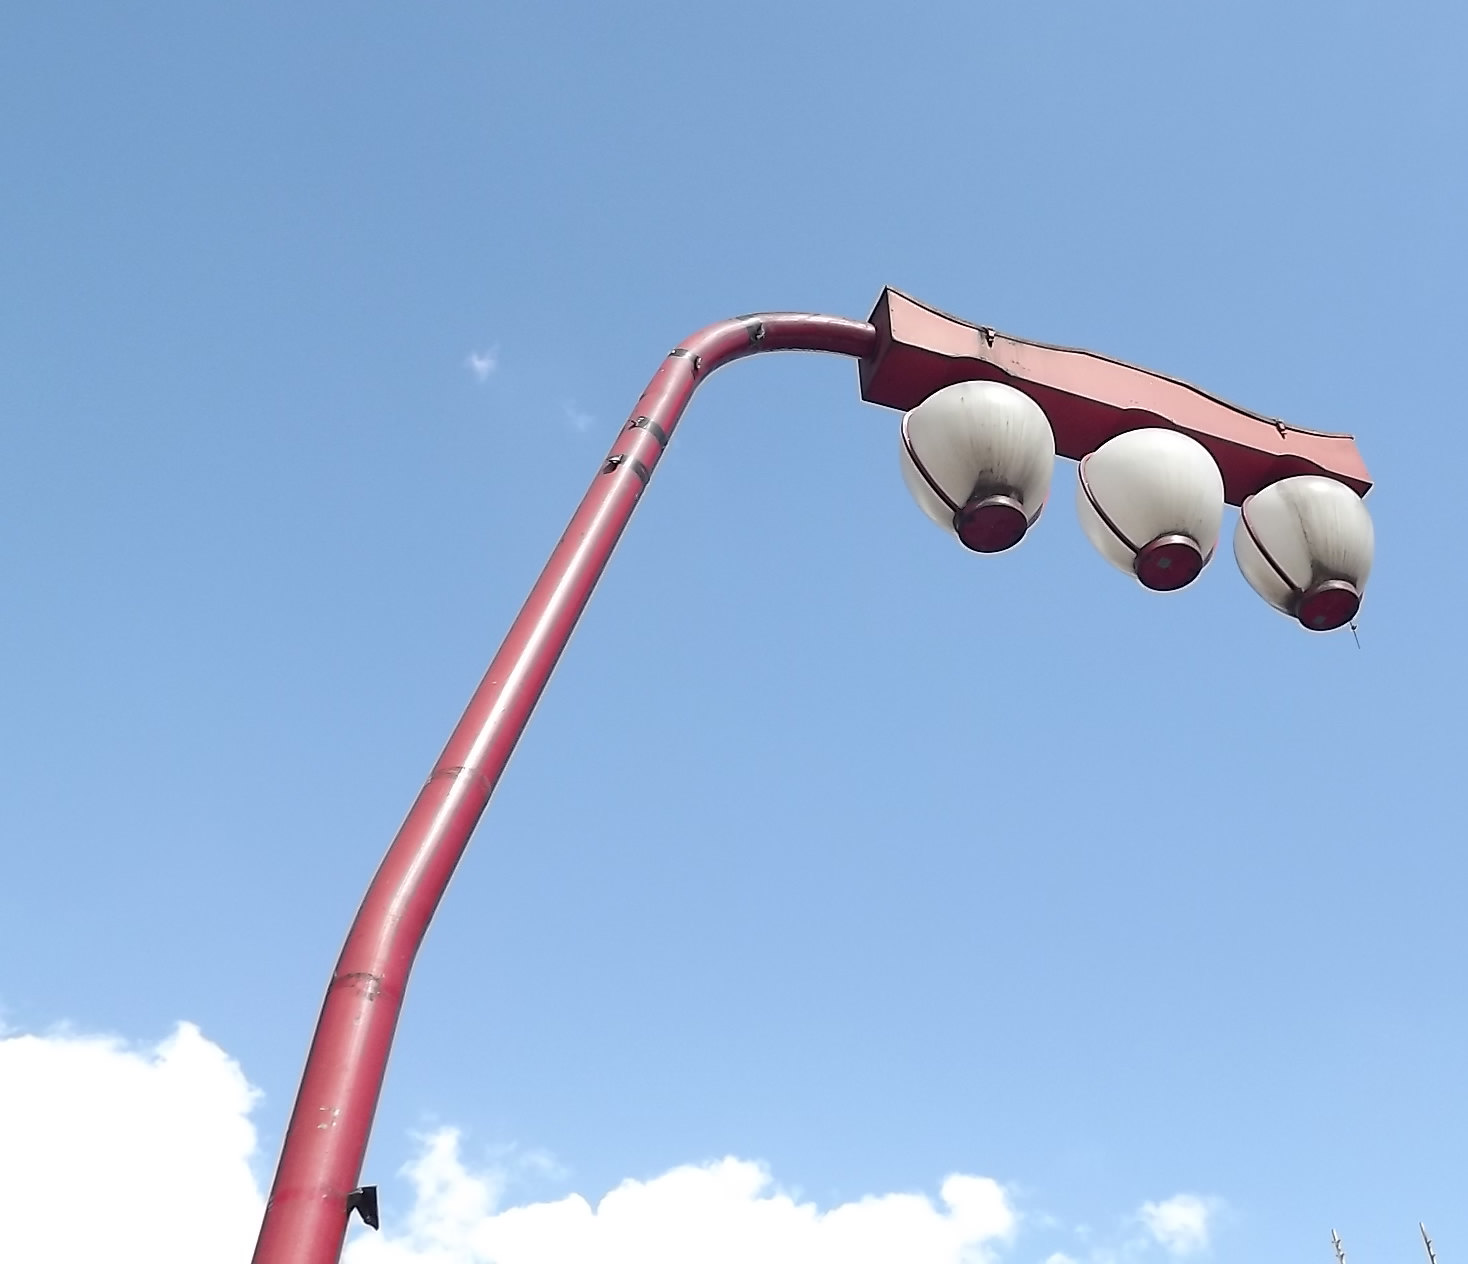
\includegraphics[width=0.3\textwidth]{assets/image_segmentation/classification_example.png}
    &
    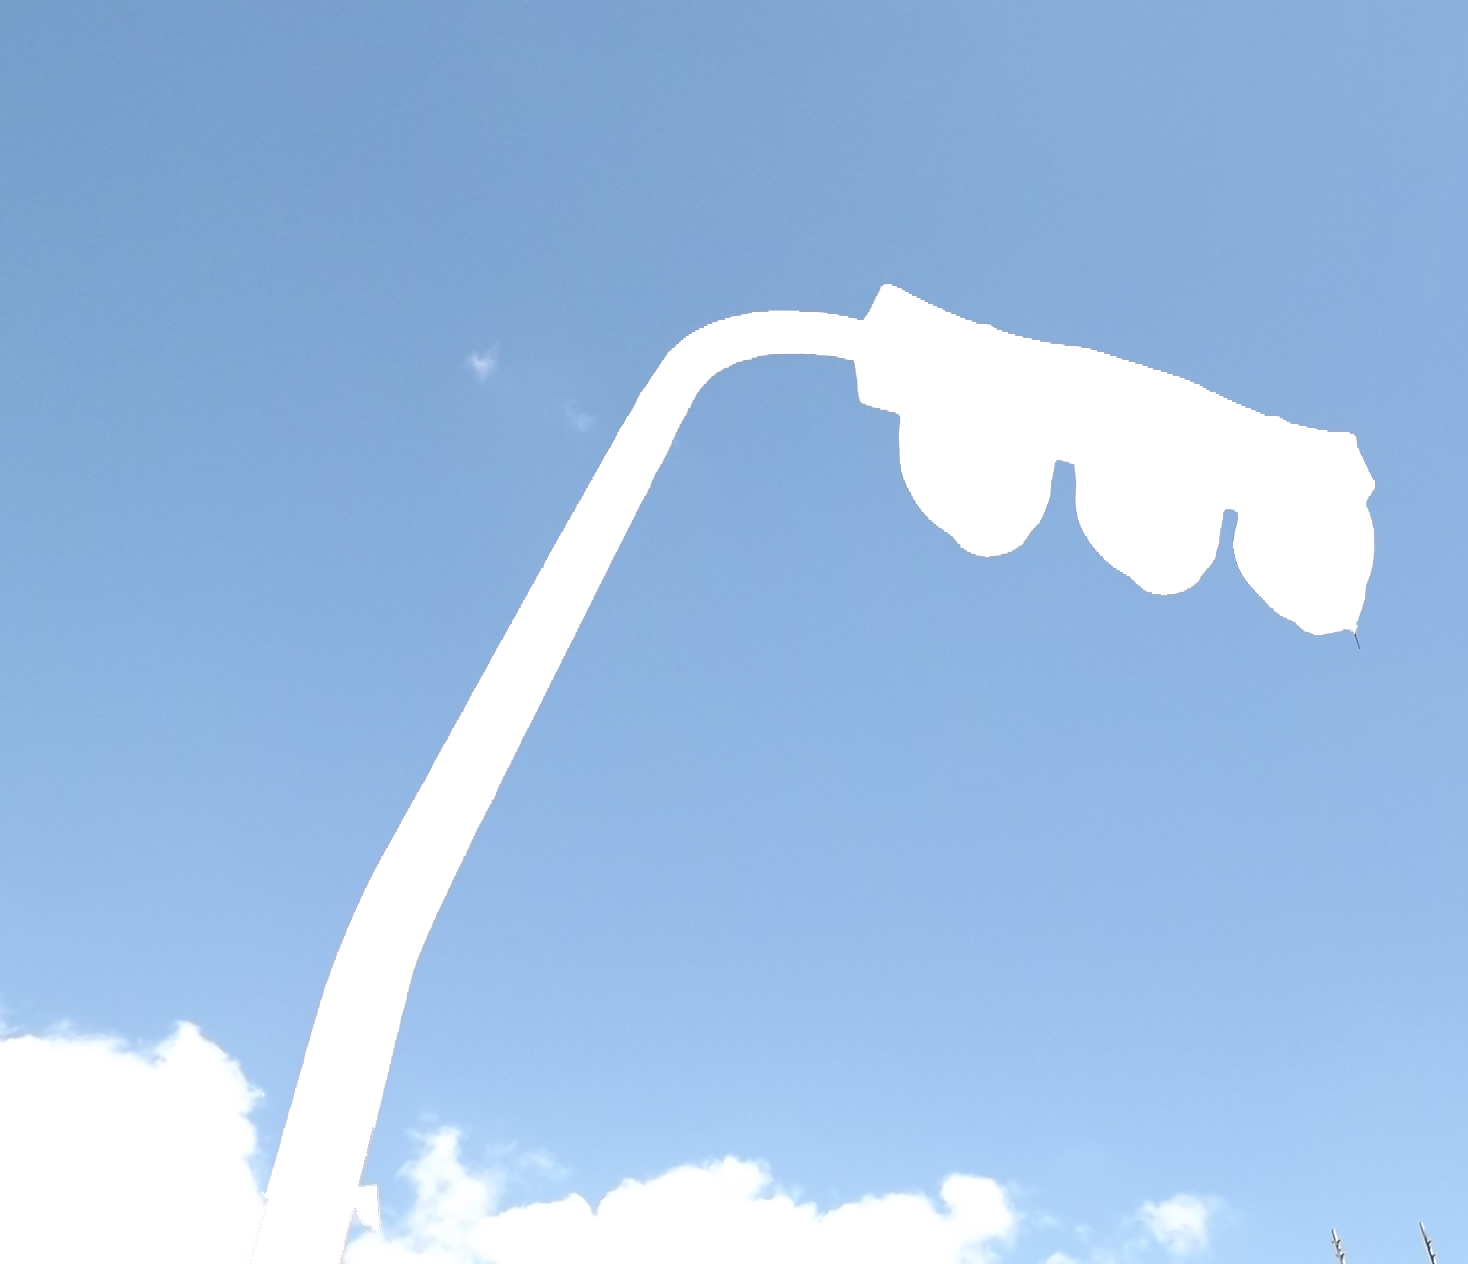
\includegraphics[width=0.3\textwidth]{assets/image_segmentation/background.png}
    &
    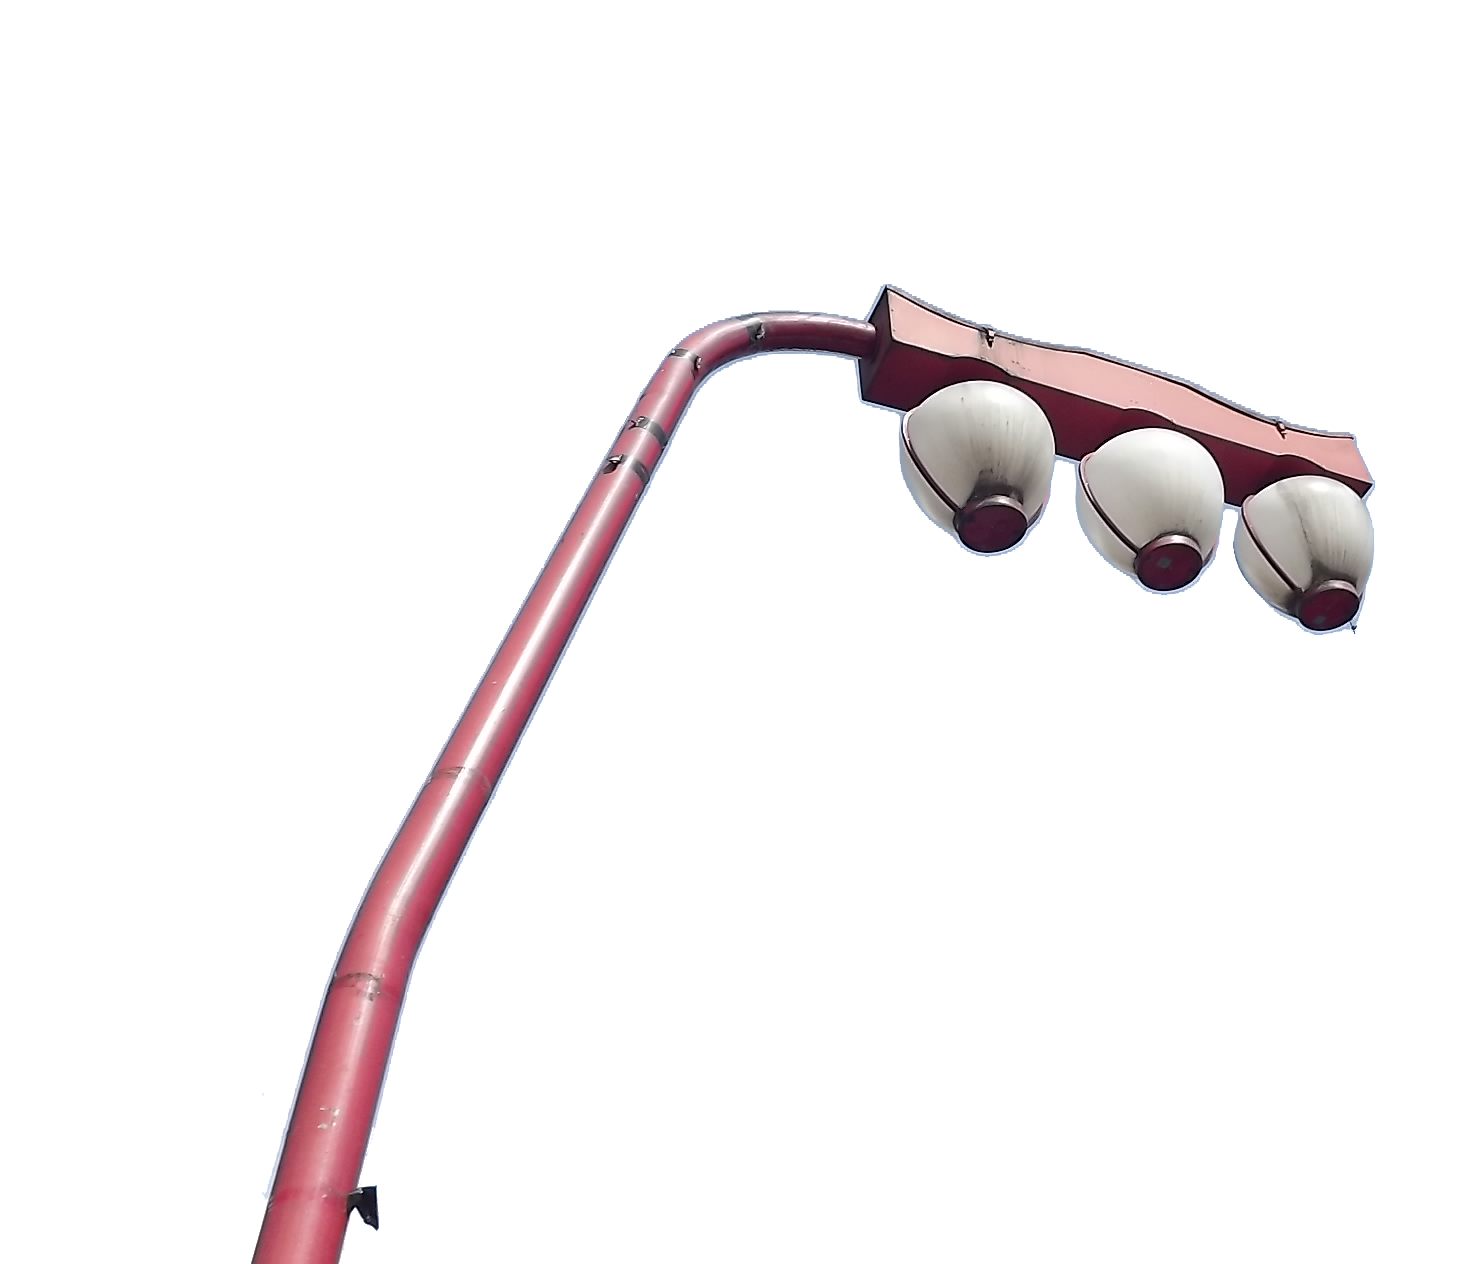
\includegraphics[width=0.3\textwidth]{assets/image_segmentation/foreground.png}
    \label{tab:image_segmentation}
  \end{tabular}
\end{table}

\subsection{Componentes de uma página}
\label{sec:components}

As componentes de interesse, o conjunto $Y$ do ponto de vista de reconhecimento de padrões, na segmentação de página são:

\begin{itemize}
  \item blocos de texto: região com parágrafos
  \item gráficos
  \item figuras
  \item títulos
  \item legendas
  \item separadores
  \item tabelas
  \item fórmulas matemáticas
  \item regiões com ruído
\end{itemize}

\subsection{Segmentação de página}

\subsection{Classificação dos componentes}

\TODO{Em outras palavras, aqui a ideia é listar as classes!}
\TODO{Aqui o ideal é explicar como a segmentação de páginas pode ser
  formulada como um porblema de classificação!}


O problema de segmentação de página pode ser descrito como o da
partição de um conjunto de pixels de uma imagem em subconjuntos. Ou
seja, dado $I = \lbrace x \colon x \in \mathbb{Z} ^ 2 \rbrace$, e um
conjunto de classes $\mathbb{C}$, a segmentação é dada por uma função

    \begin{equation}
      \begin{split}
        f \colon I &\to \mathbb{C}\\
        \cr x &\rightsquigarrow c = f(x)
      \end{split}
    \end{equation}

    % figura ilustrando a segmentação de uma imagem esquemática qualquer

    Estamos então interessados em construir uma função $f$, onde dado
    a imagem de um documento, retorne $\lbrace (x, f(x)) \rbrace$,
    $\mathbb{C}$ é o conjunto dos tipos de regiões: título, texto,
    figura, gráficos, tabelas e linhas divisoras.

    Porém, classificar cada pixel resultaria numa saída muito complexa
    e detalhada, de difícil interpretação e aplicabilidade
    prática. Assim, adotaremos uma definição mais eficiente em termos
    de utilização do espaço, de fácil compreensão e que nos
    possibilite fazer comparações entre diferentes soluções de forma
    rápida.


    Um bom equilíbrio entre flexibilidade no formato da região, custo
    de armazenamento e facilidade de interpretação é obtido com o uso
    de polígonos isotéticos. Este polígonos são formados apenas de
    linhas horizontais e verticais, envolvendo as regiões de pixels de
    uma certa classe. Ajustam-se melhor ao formato de figuras e blocos
    de texto que nem sempre são retangulares. Também podem ser
    armazenados com uma estrutura de dados eficiente em termos de
    utilização de espaço e de fácil comparação com uma outra região
    groundtruth. Este formato foi proposto no artigo [Performance
      Analysis Framework for Layout Analysis Methods].


\subsection{Avaliação da segmentação}

\TODO{Dizer aqui como se avalia uma segmentação. Poderia ser a nível
  de pixel, ou a nivel de regiões ou componentes. Pixel é fácil, mas
  tem os potenciais problemas. No caso de região é preciso definir
  como comparar regiões --- caso dos polígonos isotéticos, etc etc}






\section{Aprendizado de operadores morfológicos}

\subsection{Operadores morfológicos binários}

\TODO{Dizer o que é operador morfológico}


\subsection{Treinamento}

\TODO{Descrever o processo de treinamento}







\section{Metodologia}

\TODO{Até aqui já foi falado um pouco de PROCESSAMNTO DE IMAGENS, um
  pouco de CLASSIFICAÇÃO, um pouco sobre SEGMENTAÇÃO DE PÁGINA, e COMO
  SEGMENTAÇAO DE pÄGINA pode ser modelado como um problema de
  classificação. Foi também falado sobre OPERADORES MORFOLÓGICOS e
  como se faz seu treinamento.}

\TODO{Aqui deve ser dito como essas coisas se encaixam. Ou seja, é
  mais ou menos o que você faz aqui, de descrever o processo. Mas, na
  medida do possível, deve-se transferir definições, conecitos,
  algoritmos, etc para as partes anteriores. Aqui deve-se relatar o
  processo e qual método/técnica/algoritmo é usado no processo. A
  descrição dos parâmatros efetivamente usados deve ser apresentado na
seção de experimentos.}.

O método empregado para resolver o problema é baseado em operadores morfológicos automaticamente gerados. Algumas etapas de pré e pós processamentos também foram necessárias para preparar a entrada e traduzir a saída do algoritmo.


\TODO{ESSE parágrafo é o tipo de informação que poderia estar na
  INTRODUÇÃO, como parte de motivação e justificativa do trabalho.}
Construir operadores morfológicos que resolvam problemas complexos como o de segmentar uma página de documento, pode ser uma tarefa que demande muito tempo, experiência e conhecimento específico do assunto. Como estas imagens possuem características distintas dependendo da publicação, é possível que apenas um operador não consiga ser aplicado a todas as imagens. Ou seja, construir operadores com facilidade é um fator sensível para a escolha desta abordagem.


    O processo é organizado nas seguintes etapas:

    \begin{enumerate}
      \item Aquisição das imagens de treinamento
      \item Binarização
      \item Construção do operador segmentador específico para o tipo de região especificada
      \item Aplicação do operador em um conjunto de imagens
      \item Pós-processamentos
      \item Definição dos polígonos delimitadores de regiões
    \end{enumerate}

    Cada um dos passos é detalhado nas seções seguintes.

    \subsection{Aquisição das imagens de treinamento}

      As imagens utilizadas nos experimentos foram obtidas de um banco de dados construído pelos pesquisadores do PRImA ao longo de anos. Ele inclui um conjunto de documentos que busca simular um cenário realístico de trabalho, com layouts complexos e diferentes tipos de fontes e formatos de regiões. Isto é importante para avaliar a aplicabilidade do método em situações práticas, onde um controle sobre o formato do conteúdo seria indesejável ou inviável.

      No artigo [A Realistic Dataset for Performance Evaluation of Document Layout Analysis] de 2009, os autores apresentam um conjunto de dados com páginas de revistas, artigos científicos diversos, documentos modernos e não apenas históricos.

      O conjunto de dados contém não só imagens mas também arquivos XML [The PAGE (Page Analysis and Ground-truth Elements) Format Framework] com metadados como informações bibliográficas (título, autor, publicação), informações das imagens (resolução, bit depth, modelo do scanner), características do layout (número de colunas, variadade de tamanhos de fontes) e informações administrativas (direitos autorais).

      Os documentos são digitalizados com um cartão escuro por trás para minimizar a exposição da contra página. Posteriormente um algoritmo analisa possíveis falhas, como rotação do documento, marcando-os para redigitalização. Uma correção automática não é utilizada pois isto pode comprometer a qualidade da imagem.

      Uma vez que a imagem foi aceita no banco de dados, inicia-se um processo manual de marcação do grownd-truth. Este trabalho deve ser realizado da forma mais precisa possível pois é a base para determinar a corretude dos algoritmos segmentadores. Por se tratar de uma etapa muito custosa, uma ferramenta semi-automática chamada Aletheia é utilizada para agilizar o processo. Esta ferramenta permite a uma pessoa desenhar uma região poligonal em torno de uma região de interesse. Em seguida esta região é automaticamate ajustada pelo software, como se a pessoa estivesse colocando um elástico que aperta a região.

      As imagens utilizadas para exemplificação nesta monografia não são as mesmas do banco de dados referido por limitações de licença.

    \subsection{Algoritmo de Otsu para binarização}

      \TODO{Colocar pseudo-código?}

      % O processo de transformar uma imagem colorida em uma imagem binária simplifica a imagem, ou seja, destrói informação. Esta perda pode comprometer todas as etapas subsequêntes caso não seja feita de forma apropriada.

      Implementar e avaliar cada algoritmo binarizador vai além do escopo deste trabalho, portanto escolhemos um bom algoritmo segundo os resultados obtidos em \cite{citeulike:890354}. Como o próprio artigo aponta, não foi encontrado um método que apresentasse desempenho superior em todas os cenários de teste realizados.

      Os requisitos para a escolha foram o da independência de supervisionamento e parametrização. Caso o algoritmo demandasse ajustes específicos de acordo com a imagem, o seu uso comprometeria a promissa de automatização. Dentre a lista de soluções com esta característica, escolhemos o algoritmo de Otsu \cite{1979:ots}, por ser de fácil implementação e apresentar resultados satisfatórios nos experimentos realizados.

      O algoritmo de Otsu encontra um nível de cinza $t$ tal que a soma ponderada da variância dentro das classes $\mathbb{F} = \{ x \colon f(x) \geq t \}$ (foreground) e $\mathbb{B} = \{ x \colon f(x) < t \}$ (background) seja minimizada, ou seja,

      \begin{equation}
        t = argmin \{ w_\mathbb{B} \sigma^{2}_{\mathbb{B}} + w_\mathbb{F} \sigma^{2}_{\mathbb{F}} \}
      \end{equation}

      onde $w_\mathbb{B} = \frac{|\mathbb{B}|}{|E|}$ e $w_f = \frac{|\mathbb{F}|}{|E|}$ são os pesos respectivamente do background e foreground e $\sigma^{2}_{\mathbb{B}}$ e $\sigma^{2}_{\mathbb{F}}$ são as variâncias das classes.

      A tabela \ref{tab:otsu} apresenta um passo a passo do algoritmo aplicado à figura \ref{fig:letrah}.

      \begin{figure*}[htb]
        \begin{center}
          
\includegraphics[width=0.5\textwidth]{assets/binarization/h_3grayscale_big.png}
          \end{center}
        \caption{Imagem digitalizada de uma letra H obtida de uma revista.}
        \label{fig:letrah}
      \end{figure*}

      \begin{center}

      \begin{table}
        \caption{Estágios da execução do algoritmo de Otsu.}
        \begin{tabular}[p]{@{}ccccccc@{}}
          \centering

          original & 25\% & 37,5\% & 50\% & 62,5\% & 75\% & 87,5\% \\

          % Imagem original e respectivo histograma
          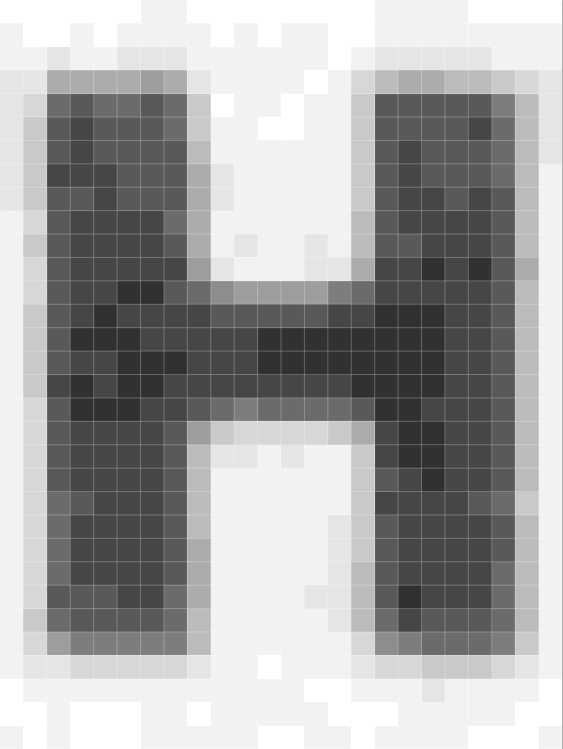
\includegraphics[width=0.05\textwidth]{assets/binarization/gray3_big.png}
          &
          
\includegraphics[width=0.05\textwidth]{assets/binarization/h25t.png}
          &
          
\includegraphics[width=0.05\textwidth]{assets/binarization/h38t.png}
          &
          
\includegraphics[width=0.05\textwidth]{assets/binarization/h50t.png}
          &
          
\includegraphics[width=0.05\textwidth]{assets/binarization/h63t.png}
          &
          
\includegraphics[width=0.05\textwidth]{assets/binarization/h75t.png}
          &
          
\includegraphics[width=0.05\textwidth]{assets/binarization/h88t.png}
          \\

          % histogramas

          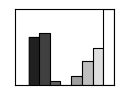
\includegraphics[scale=0.4]{assets/binarization/3bit_hist.png}
          &
          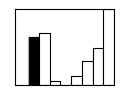
\includegraphics[scale=0.4]{assets/binarization/13hist.png}
          &
          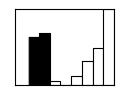
\includegraphics[scale=0.4]{assets/binarization/25hist.png}
          &
          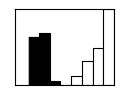
\includegraphics[scale=0.4]{assets/binarization/50hist.png}
          &
          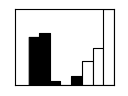
\includegraphics[scale=0.4]{assets/binarization/63hist.png}
          &
          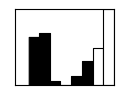
\includegraphics[scale=0.4]{assets/binarization/75hist.png}
          &
          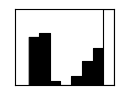
\includegraphics[scale=0.4]{assets/binarization/88hist.png}

          \\
          % peso do background
          $w_\mathbb{B}$ & 0.1931 & 0.4015 & 0.4179 & 0.4532 & 0.5479 & 0.6969 \\

          % média do background
          $\mu_\mathbb{B}$ & 34.00 & 51.64 & 53.61 & 61.37 & 83.08 & 112.56 \\

          % variância do background
          $\sigma^{2}_{\mathbb{B}}$ & 7.27 & 288.58 & 372.94 & 1054.08 & 3128.03 & 5656.37 \\

          % peso do foreground
          $w_{\mathbb{F}}$ & 0.80 & 0.59 & 0.58 & 0.54 & 0.45 & 0.30 \\

          % média do foreground
          $\mu_{\mathbb{F}}$ & 184.87 & 225.55 & 229.03 & 233.95 & 243.79 & 255.0 \\

          % variância do foreground
          $\sigma^{2}_{\mathbb{F}}$ & 5799.89 & 1409.01 & 1006.11 & 673.10 & 255.43 & 0.0 \\

          % variância intra-classe
          $\sigma^{2}_{w}$ & 21495165144 & 967521582 & 512693389 & 595067475 & 4269882800 & 17660993341 \\

          \label{tab:otsu}
        \end{tabular}
      \end{table}
      \end{center}

      Como podemos notar, para $t = 50\%$ atingimos o menor valor de $\sigma^{2}_{w} \approx 512693389$. Neste caso o limiar coincide com o único vale no histograma, porém isto nem sempre será válido. Algumas imagens não possuem vales bem definidos. Este algoritmo não se baseia no formato do histograma mas sim na coesão intra classe e na separabilidade das classes.

      \begin{figure*}[htb]
        \begin{center}
          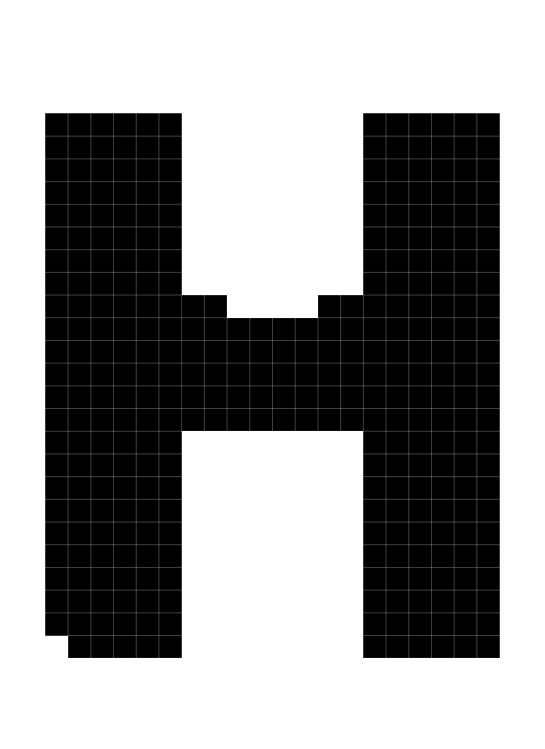
\includegraphics[width=0.5\textwidth]{assets/binarization/bin_big.png}
          \end{center}
        \caption{Imagem binarizada com $t = 50\%.$}
        \label{fig:letrah_bin}
      \end{figure*}

      Uma desvantagem de utilizar este algoritmo é a influência da média de todo os pixels da imagem. Isto pode fazer com que o limiar ótimo para a página toda não seja o mesmo que o de dentro de uma janela.

      % 
      % Usei o imagemagick para criar uma imagem em tons de cinza com a quantidade de níveis desejado, usando o seguinte comando
      % 
      % convert -type Grayscale -depth 3 h8rgb.png h_3grayscale.png
      % 
      % Posteriormente gerei imagens com threshold em diferentes níveis
      % 
      % convert -threshold 60% h_3grayscale.png h60t.png
      % 
      % o comando identify -verbose mostra o histograma
      % 
      % Usei o gráfico do site http://www.labbookpages.co.uk/software/imgProc/otsuThreshold.html como exemplo
      % 
      % binarizado com ../otsuthresh -g save h_3grayscale.png bin.gif
      % 

    \subsection{Construção do operador}

      O algoritmo gerador de operadores morfológicos recebe como entrada duas imagens, uma é chamada de original e consiste da imagem branco e preto resultante da binarização e a segunda, chamada de alvo, é uma transformação da imagem original. Esta transformação é feita manualmente e procura demonstrar o conceito de segmentação para o algoritmo de treinamento.

      % não sei se em algum momento devo apresentar uma definição mais formal de machine learning. Me lembro de ter lido algo na tese. Era complicado.

      De posse apenas da imagem original, devemos gerar a imagem de destino aplicando uma transformação adequada. Neste ponto exploraremos algumas estratégias diferentes revelando pontos positivos e negativos de se usar esta abordagem.

      \subsubsection{Apagar área de interesse}

        Nossa primeira estratégia foi apagar as regiões indicadas, pintando-as de branco. Partindo da premissa de que o operador gerado seria o ótimo para este tipo de transformação, poderíamos obter os pixels em regiões do tipo especificado ao fazer a diferença entre a imagem de entrada e a de saída.

      \subsubsection{Pintar área de interesse}

        Preenchemos todos os pixels das regiões indicadas, pintando-a completamente. Apagamos todos os demais. Desta forma poderíamos produzir componentes conexos com os pixels de uma certa região.

      \subsubsection{Manter apenas área de interesse}

        Apagamos toda a imagem exceto a região de interesse. Desta forma procuramos construir um operador preserve apenas os pixels da área de interesse, porém sem aglutiná-los, como na estratégia anterior.

      \subsubsection{Aprendizado iterativo}

        No caso de a abordagem anterior gerar um operador cujo MAE seja insatisfatório, podemos gerar outro operador a partir da imagem processada e a imagem ideal, novamente. Esta técnica funciona como um reforço.

      \subsubsection{Diminuir resolução}

        Reduzimos a resolução da imagem reduzindo a complexidade das formas e o tempo de processamento para construção do operador. Esta técnica é especialmente útil para o tratamento de títulos.

    \subsection{Pós processamento}

      O operador gerado na etapa anterior é uma aproximação de um operador considerado ideal. A aplicação deste operador produz resultados considerados sub ótimos. Após realizar experimentar com as diferentes estratégias citadas anteriormente e também com diferentes tamanhos de janela, observamos que as imagens produzidas poderiam ser melhoradas com técnicas simples.

      Buscando complementar a transformação, adicionamos mais alguns passos, descritos a seguir.

      \subsubsection{Reconstrução de pixels na área de interesse parcialmente apagada}

        Caso o operador apague alguns pixels de uma componente conexa, mas não apague a componente toda, recuperamos a componente a partir dos pixels restantes e da imagem original.

      \subsubsection{Unir pixels de uma região em componentes conexas}

        Para facilitar a definição do polígono que envolve uma região, aplicamos um operador que aglutina as componentes remanescentes.

    \subsection{Definição dos polígonos delimitadores de regiões}

      Definir pontos do polígono que envolve cada componente conexa.

    \subsection{Análise do desempenho}

      O PRImA disponibiliza um software que implementa o algoritmo de comparação descrito em [Scenario Driven In-Depth Performance Evaluation of Document Layout Analysis Methods].

      A comparação entre a solução obtida e a solução ideal, é dividida nas seguintes situações:

      \begin{itemize}
        \item a região segmentada não possui intersecção alguma com as regiões growndtruth.
        \item a região growndtruth é totalmente coberta pela região segmentada.
        \item a região growndtruth é coberta por duas regiões segmentadas, dividindo-a.
        \item duas regiões growdtruth são unidas por uma única região segmentada.
        \item uma região growndtruth não é coberta por nenhuma região segmentada, ou seja, esquecida.
      \end{itemize}

      A importância de cada erro ou acerto pode ser contextualizado de acordo com o problema em questão. Por exemplo, a união de duas regiões growntruth em uma única região segmentada pode não ser um erro indesejável caso a ordem de leitura seja respeitada.





\section{Resultados experimentais}

Nesta seção serão descritos os resultados experimentais obtidos.

\subsection{Base de dados}
Descrever a base de imagens utilizadas.

Qual pré-processamento foi aplicado e com quais parâmetros.


\subsection{Experimento A}

\subsection{Experimento B}


\subsection{Discussão}

      \begin{itemize}
        \item Estatísticas com base no MAE das estratégias propostas.
        \item Estatísticas do ICDAR.
      \end{itemize}



\section{Conclusão}




\section{Apêndice}

\subsection{TRIOS}

\TODO{O TRIOS é apenas uma implementação do processo de treinamento de
  operadores morfológicos. Assim, se for para colocar isso na
  monografia, acho que deveria estar no Apêndice.}
      \begin{itemize}
        \item Imagem enquanto conjunto ou função
        \item Transformação entre conjuntos
        \item Exemplos: dilatação, erosão, abertura, fechamento, gradiente, hit-or-miss, sup-gerador.
        \item Operadores invariantes por translação e localmente definidos.
        \item W-Operadores.
        \item Teorema da decomposição canônica (não sei quanto disto eu consigo explicar).
        \item Conjuntos aleatórios S e I. Caracterização por um processo estacionário local (X, y).
        \item Otimalidade de Psy com base num operador localmente definido (MAE).
        \item Algoritmo: Estimativa de P(y | X), decisão, generalização (ISI?).
        \item Bias-Variance Tradeoff
        \item Explorando estrutura de Psy? (talvez isso caiba melhor na lista de estratégias a seguir)
        \item Escolha da janela ótima.
        \item Operador multi-nível.
      \end{itemize}

      %% \subsubsection{Álgebra booleana}

      %% Definições básicas até minimização de expressões.

      %% \subsubsection{Probabilidade}

      %% \begin{itemize}
      %%   \item Espaço amostral, eventos, etc
      %%   \item FDP
      %%   \item Probabilidade conjunta e condicional
      %%   \item Variável aleatória
      %%   \item Experança estatística
      %%   \item Processo estacionário
      %% \end{itemize}

%\bibliographystyle{alpha}
{\small 
\bibliographystyle{unsrt} % (uses file "plain.bst")
\bibliography{myrefs}   % expects file "myrefs.bib"
}

\end{document}
